\documentclass[a4paper,11pt]{report}\usepackage[]{graphicx}\usepackage[]{color}
%% maxwidth is the original width if it is less than linewidth
%% otherwise use linewidth (to make sure the graphics do not exceed the margin)
\makeatletter
\def\maxwidth{ %
  \ifdim\Gin@nat@width>\linewidth
    \linewidth
  \else
    \Gin@nat@width
  \fi
}
\makeatother

\definecolor{fgcolor}{rgb}{0.345, 0.345, 0.345}
\newcommand{\hlnum}[1]{\textcolor[rgb]{0.686,0.059,0.569}{#1}}%
\newcommand{\hlstr}[1]{\textcolor[rgb]{0.192,0.494,0.8}{#1}}%
\newcommand{\hlcom}[1]{\textcolor[rgb]{0.678,0.584,0.686}{\textit{#1}}}%
\newcommand{\hlopt}[1]{\textcolor[rgb]{0,0,0}{#1}}%
\newcommand{\hlstd}[1]{\textcolor[rgb]{0.345,0.345,0.345}{#1}}%
\newcommand{\hlkwa}[1]{\textcolor[rgb]{0.161,0.373,0.58}{\textbf{#1}}}%
\newcommand{\hlkwb}[1]{\textcolor[rgb]{0.69,0.353,0.396}{#1}}%
\newcommand{\hlkwc}[1]{\textcolor[rgb]{0.333,0.667,0.333}{#1}}%
\newcommand{\hlkwd}[1]{\textcolor[rgb]{0.737,0.353,0.396}{\textbf{#1}}}%

\usepackage{framed}
\makeatletter
\newenvironment{kframe}{%
 \def\at@end@of@kframe{}%
 \ifinner\ifhmode%
  \def\at@end@of@kframe{\end{minipage}}%
  \begin{minipage}{\columnwidth}%
 \fi\fi%
 \def\FrameCommand##1{\hskip\@totalleftmargin \hskip-\fboxsep
 \colorbox{shadecolor}{##1}\hskip-\fboxsep
     % There is no \\@totalrightmargin, so:
     \hskip-\linewidth \hskip-\@totalleftmargin \hskip\columnwidth}%
 \MakeFramed {\advance\hsize-\width
   \@totalleftmargin\z@ \linewidth\hsize
   \@setminipage}}%
 {\par\unskip\endMakeFramed%
 \at@end@of@kframe}
\makeatother

\definecolor{shadecolor}{rgb}{.97, .97, .97}
\definecolor{messagecolor}{rgb}{0, 0, 0}
\definecolor{warningcolor}{rgb}{1, 0, 1}
\definecolor{errorcolor}{rgb}{1, 0, 0}
\newenvironment{knitrout}{}{} % an empty environment to be redefined in TeX

\usepackage{alltt}
\usepackage{polyglossia}
\usepackage{fontspec}
\setmainfont{Times New Roman}

%%% Проверка используемого TeX-движка %%%
\usepackage{ifxetex}

%%% Поля и разметка страницы %%%
\usepackage{lscape}                                 % Для включения альбомных страниц
\usepackage{geometry}                               % Для последующего задания полей

%%% Математические пакеты %%%
%\usepackage{amsthm,amsfonts,amsmath,amssymb,amscd}  % Математические дополнения от AMS
\usepackage{amsfonts,amsmath,amssymb,amscd} %edited to knitr compatibility


%%% Кодировки и шрифты %%%
\usepackage{polyglossia}                          % Поддержка многоязычности
\usepackage{fontspec}                             % TrueType-шрифты

%%% Оформление абзацев %%%
\usepackage{indentfirst}                            % Красная строка

%%% Цвета %%%
%\usepackage[usenames]{color}
%\usepackage{color}
%\usepackage{colortbl}

%%% Таблицы %%%
\usepackage{longtable}                              % Длинные таблицы
\usepackage{multirow,makecell,array}                % Улучшенное форматирование таблиц

%%% Общее форматирование
\usepackage[singlelinecheck=off,center]{caption}    % Многострочные подписи
\usepackage{soul}                                   % Поддержка переносоустойчивых подчёркиваний и зачёркиваний
\usepackage{icomma}                                 % Запятая в десятичных дробях

%%% Библиография %%%
\usepackage{cite}                                   % Красивые ссылки на литературу

%%% Гиперссылки %%%
\usepackage[linktocpage=true,plainpages=false,pdfpagelabels=false]{hyperref}

%%% Изображения %%%
\usepackage{graphicx,wrapfig}                              % Подключаем пакет работы с графикой

%%% Оглавление %%%
\usepackage{tocloft}

%%% Интервалы %%%
\usepackage{setspace}

%%% Колонтитулы %%%
\usepackage{fancyhdr}
       
%%% Макет страницы %%%
% Выставляем значения полей (ГОСТ 7.0.11-2011, 5.3.7)
\geometry{a4paper,top=2cm,bottom=2cm,left=2.5cm,right=1cm}

%%% Кодировки и шрифты %%%
\ifxetex
  \setmainlanguage{russian}
  \setotherlanguage{english}
  \defaultfontfeatures{Ligatures=TeX,Mapping=tex-text}
  \setmainfont{Times New Roman}
  \newfontfamily\cyrillicfont{Times New Roman}
  \setsansfont{Arial}
  \newfontfamily\cyrillicfontsf{Arial}
  \setmonofont{Courier New}
  \newfontfamily\cyrillicfonttt{Courier New}
\else
  \IfFileExists{pscyr.sty}{\renewcommand{\rmdefault}{ftm}}{}
\fi

%%% Интервалы %%%
\linespread{1.3}                    % Полуторный интвервал (ГОСТ Р 7.0.11-2011, 5.3.6)

%%% Выравнивание и переносы %%%
\sloppy                             % Избавляемся от переполнений
\clubpenalty=10000                  % Запрещаем разрыв страницы после первой строки абзаца
\widowpenalty=10000                 % Запрещаем разрыв страницы после последней строки абзаца

%%% Библиография %%%
\makeatletter
\bibliographystyle{utf8gost71u}     % Оформляем библиографию по ГОСТ 7.1 (ГОСТ Р 7.0.11-2011, 5.6.7)
\renewcommand{\@biblabel}[1]{#1.}   % Заменяем библиографию с квадратных скобок на точку
\makeatother

%%% Изображения %%%
\graphicspath{{images/}}            % Пути к изображениям

%%% Цвета гиперссылок %%%
\definecolor{linkcolor}{rgb}{0.9,0,0}
\definecolor{citecolor}{rgb}{0,0.6,0}
\definecolor{urlcolor}{rgb}{0,0,1}
\hypersetup{
    colorlinks, linkcolor={linkcolor},
    citecolor={citecolor}, urlcolor={urlcolor}
}

%%% Оглавление %%%
\renewcommand{\cftchapdotsep}{\cftdotsep}

%%% Шаблон %%%
\newcommand{\todo}[1]{\textcolor{red}{#1}}

%%% Списки %%%
% Используем дефис для ненумерованных списков (ГОСТ 2.105-95, 4.1.7)
\renewcommand{\labelitemi}{\normalfont\bfseries{--}} 

%%% Колонтитулы %%%
% Порядковый номер страницы печатают на середине верхнего поля страницы (ГОСТ Р 7.0.11-2011, 5.3.8)
\makeatletter
\let\ps@plain\ps@fancy              % Подчиняем первые страницы каждой главы общим правилам
\makeatother
\pagestyle{fancy}                   % Меняем стиль оформления страниц
\fancyhf{}                          % Очищаем текущие значения
\fancyhead[C]{\thepage}             % Печатаем номер страницы на середине верхнего поля
\renewcommand{\headrulewidth}{0pt}  % Убираем разделительную линию
\IfFileExists{upquote.sty}{\usepackage{upquote}}{}
\begin{document}

%==================__TITLE PAGE__===========================
\begin{titlepage}
  
\begin{center}
	НАЗВАНИЕ УЧРЕЖДЕНИЯ, В КОТОРОМ ВЫПОЛНЯЛАСЬ \\
  ДАННАЯ ЛАБОРАТОРНАЯ РАБОТА \\
\end{center}

\vspace{50mm}
\begin{center}		
  {тема: \bf \large НАЗВАНИЕ ЛАБОРАТОРНОЙ РАБОТЫ \\
	\small Лабораторная работа №12}
\end{center}
	
\vspace{30mm}	
\begin{flushright}
	Выполнил студент: \hspace{2mm} \underline{\hspace{1.2cm}} \hspace{2mm} Owen U.N. \\
	\textit{(подпись студента)} \hspace*{2cm} \\
	Группа:\hspace{0.5cm} 43426/1\par
	\vspace{2mm}
	Преподаватель:\hspace{2mm}  \underline{\hspace{1.2cm}}  \hspace{2mm} Doe J.J.\\
	\textit{(подпись преподавателя)} \hspace*{2cm} \\
\end{flushright}
	
	%\begin{figure} [h] 
	%  %\advance\rightskip-3cm
	%  \includegraphics [scale=0.23,width=0.5\textwidth, right] {title}
	%  \label{img:title}  
	%\end{figure}
	
\vspace{ \stretch{1} }
\begin{center}
	{«Санкт-Петербург»\\
		2015}
\end{center}
	
\end{titlepage}
\newpage



%==================__Test Page__===========================
\section*{Цель работы} 
Исследование однофононного резонанса, его проявления в спектре отражения полупроводника. Наблюдение и сравнение спектров отражения для разных полупроводников (на примере Ge и SiC). Освоение метода исследования спектра отражения в ИК области.

\section*{Схема установки и проведение эксперимента}
 измерение отражения SiC и Ge в диапазоне длин волн от 4 до 15 мкм;
- фиксация уровня шума (Uш) и введение соответствующих поправок;
- построение графиков измеренных спектров в осях: коэффициент отражения – длина волны, с указанием погрешностей;
- анализ спектра отражения SiC с использованием модели классического осциллятора, определение параметров модели;
- сравнение экспериментальной величины коэффициента отражения германия (средней по спектру) с расчетной. \\

\begin{wrapfigure}{r}{7.5cm}
  %\center
  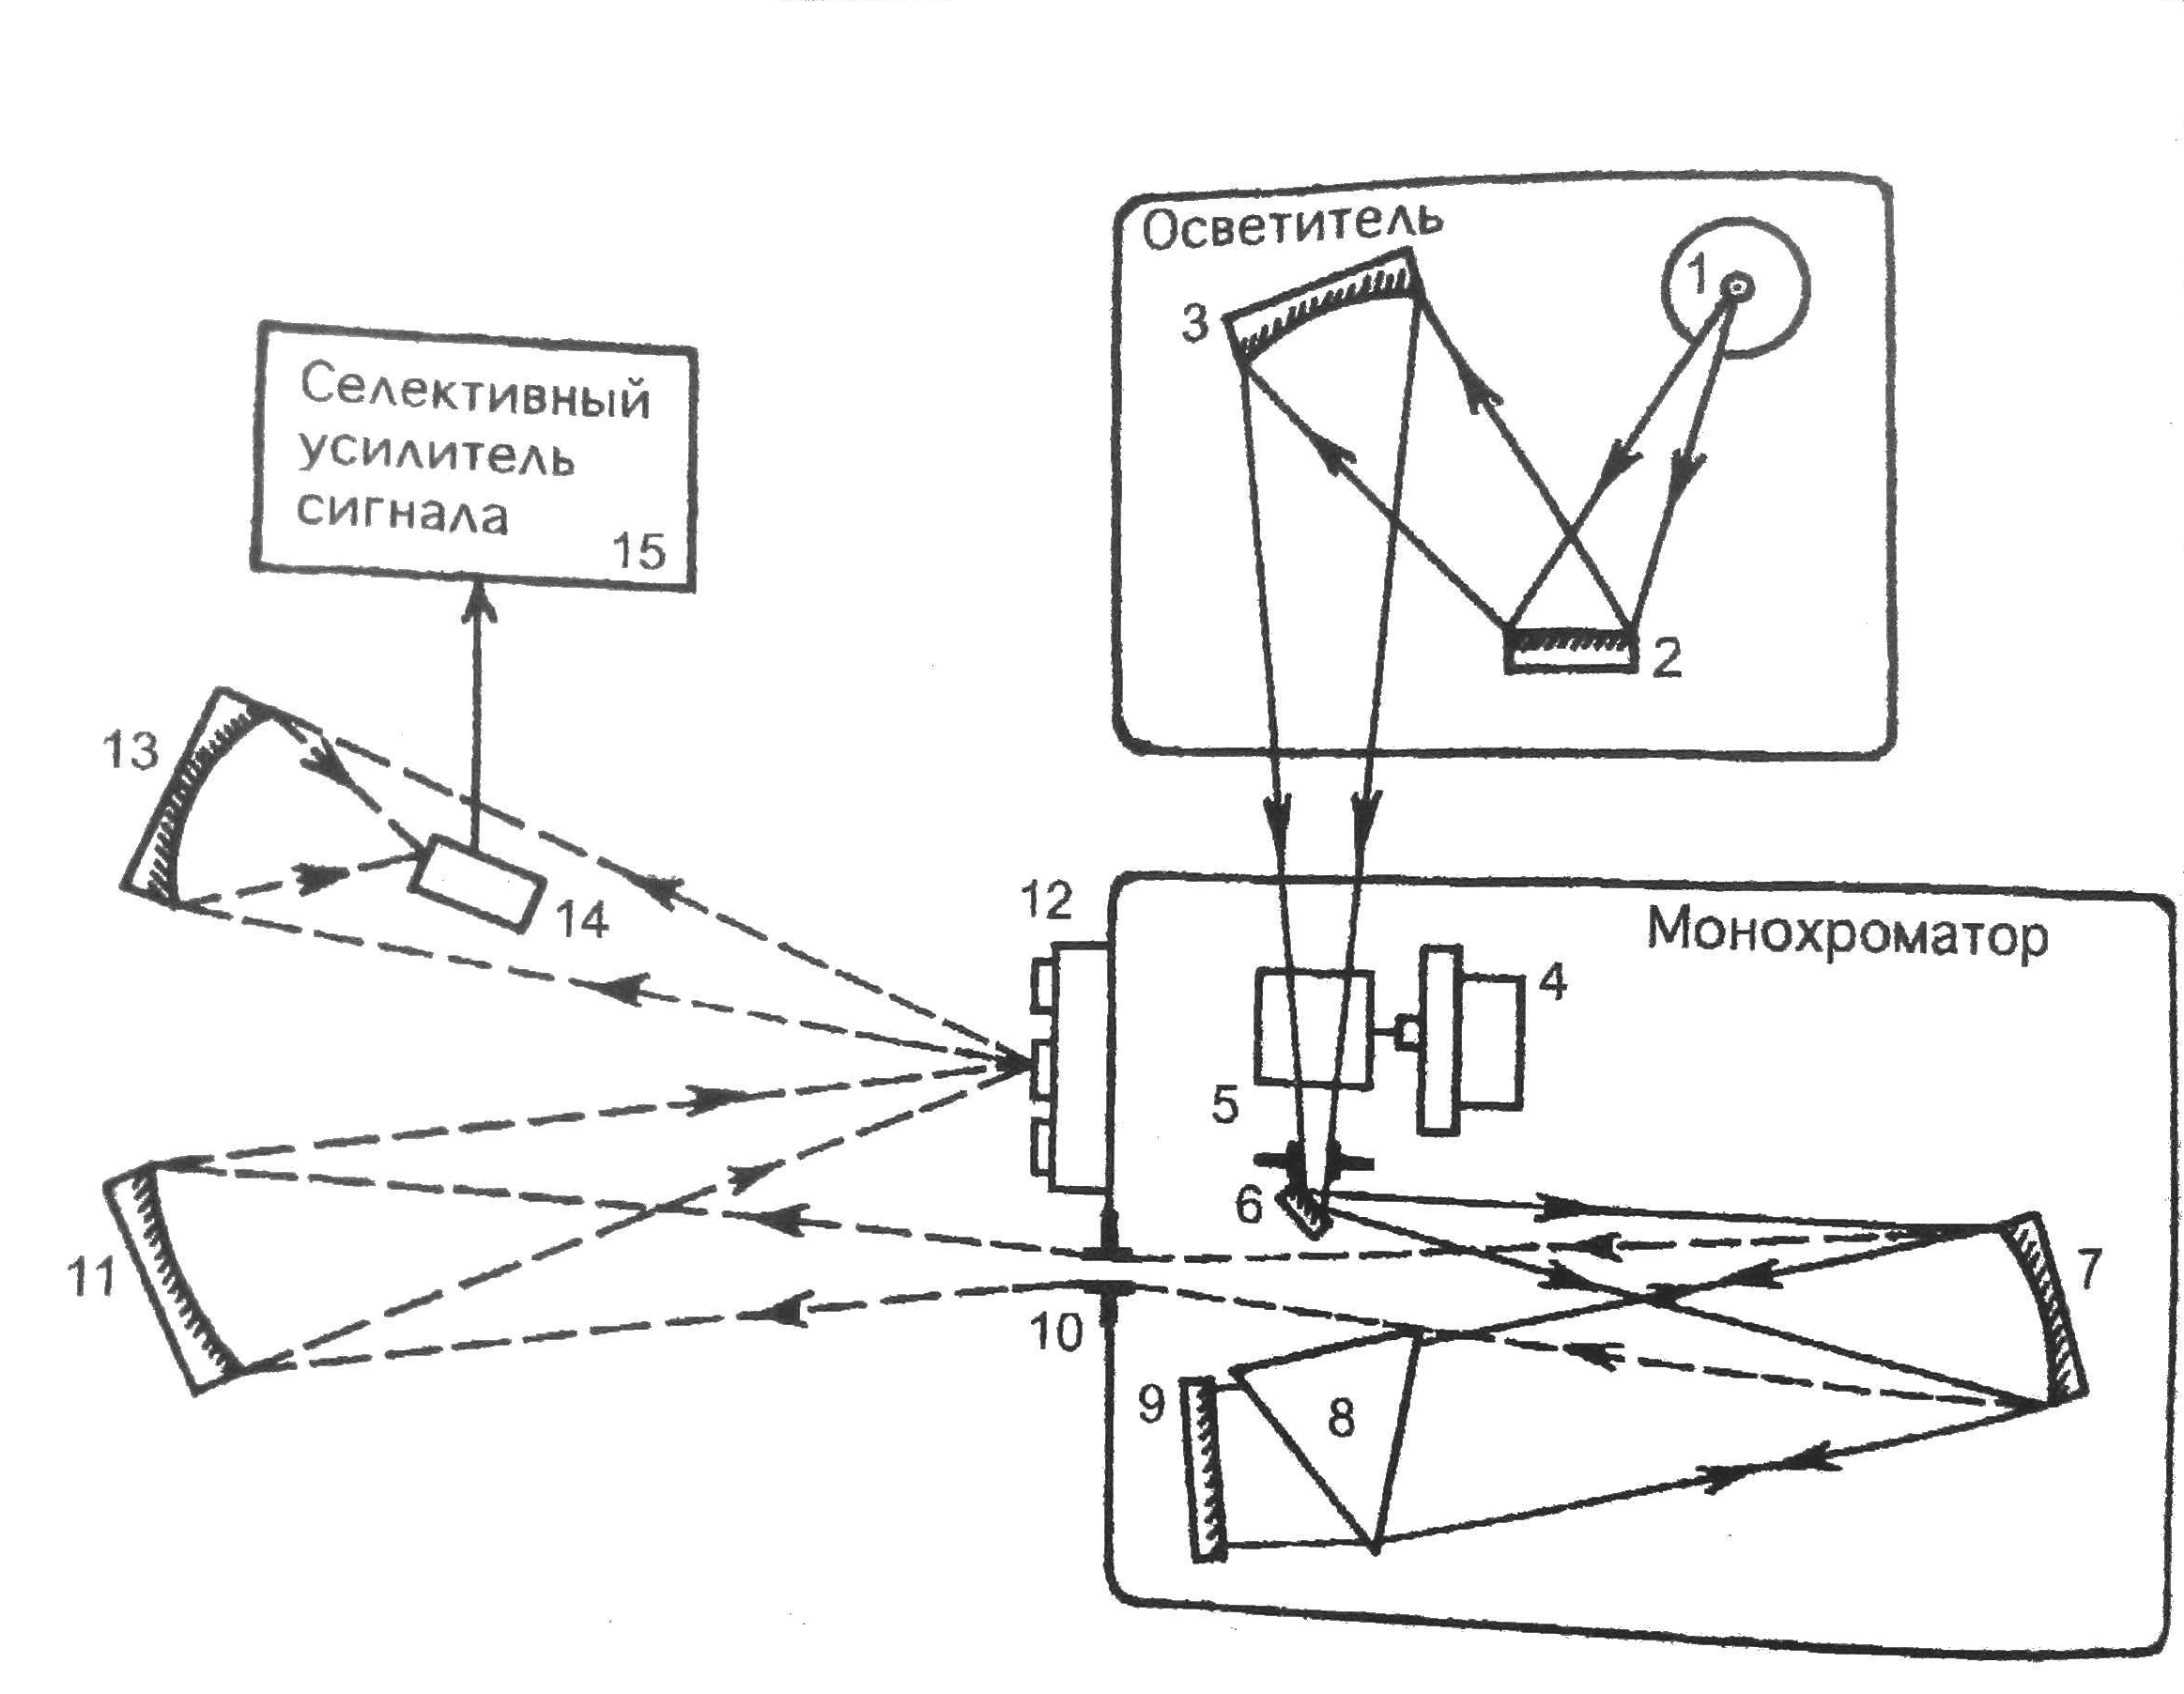
\includegraphics[width=7.5cm]{scheme}
  \caption{Схема установки} 
  \label{img:scheme}  
\end{wrapfigure} 


1. глобар \\
2. зеркало \\
3. зеркало \\
4. механический модулятор \\
5. входная щель монохроматора \\
6. плоское зеркало \\
7. параболическое зеркало \\
8. трехгранная призма \\
9. плоское зеркало \\
10. выходная щель монохроматора \\
11. сферическое зеркало \\
12. поворотная турель с образцами \\
13. сферическое зеркало \\
14. пироэлектрический фотоприемник \\
15. селективный усилитель сигнала \\


\section*{Ход работы}

% PART1 -------------------------------------------------------
\textbf{1-2.}Измерение отражения SiC и Ge

Перед проведением измерений посредством маломощной лампы накаливания была выполнена калибровка экспериментальной установки. 

Зафиксированный уровень шума много меньше измеряемого сигнала, в связи с чем данный параметр не учитывался в вычислениях.

% PART1 -------------------------------------------------------
\textbf{3.} Построим график. Рис. \ref{fig:rgraph51}

\begin{knitrout}
\definecolor{shadecolor}{rgb}{0.969, 0.969, 0.969}\color{fgcolor}\begin{kframe}


{\ttfamily\noindent\bfseries\color{errorcolor}{\#\# Error in setwd("{}\textasciitilde{}/Documents/Labs/lab08"{}): cannot change working directory}}\end{kframe}\begin{figure}[!h]
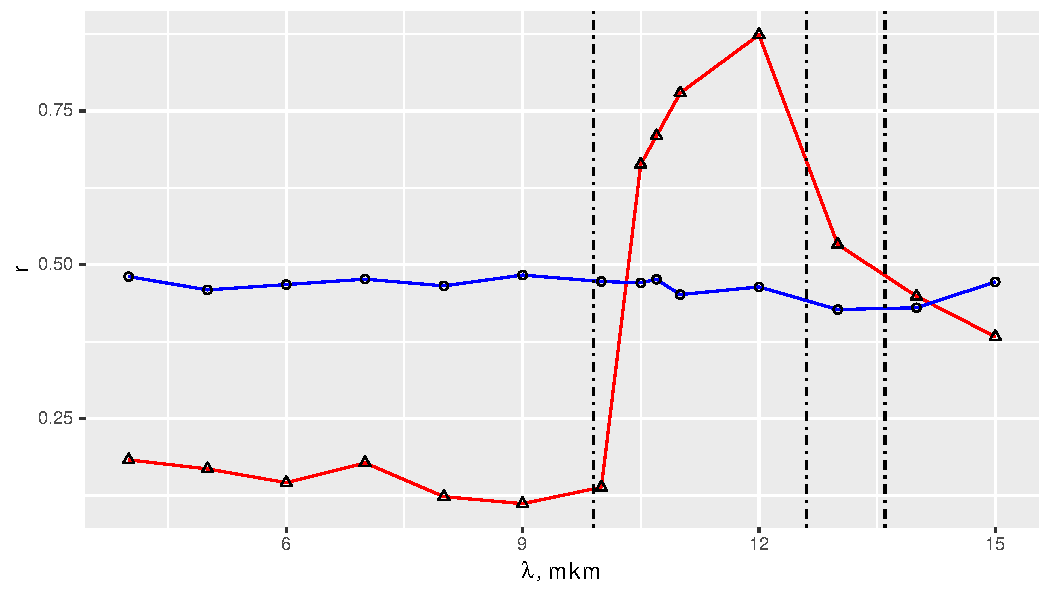
\includegraphics[width=\maxwidth]{figure/rgraph51-1} \caption[График спектров отражения]{График спектров отражения}\label{fig:rgraph51}
\end{figure}


\end{knitrout}

% PART1 -------------------------------------------------------
\textbf{4.} Проанализируем спектр отражения SiC исользуя модель классического осциллятора. Для этого перестроим график в координатах: $(1+\sqrt{r})^2/(1-\sqrt{r})^2 \sim 1/(\lambda^2-\lambda_0^2) $


\begin{knitrout}
\definecolor{shadecolor}{rgb}{0.969, 0.969, 0.969}\color{fgcolor}\begin{kframe}


{\ttfamily\noindent\bfseries\color{errorcolor}{\#\# Error in setwd("{}\textasciitilde{}/Documents/Labs/lab08"{}): cannot change working directory}}\end{kframe}\begin{figure}[!h]
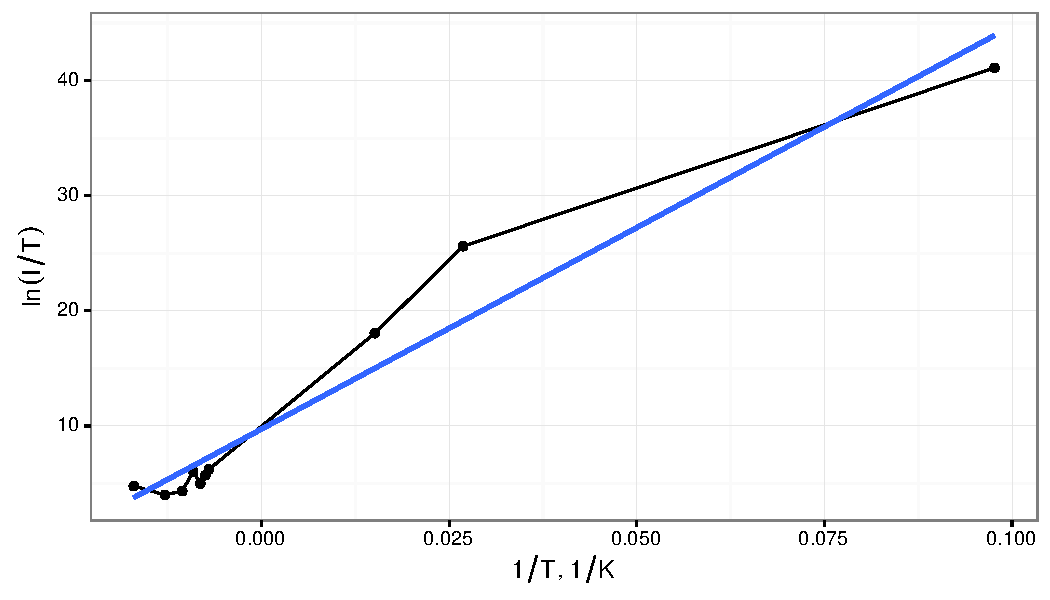
\includegraphics[width=\maxwidth]{figure/rgraph52-1} \caption[Перестроенный спектр ]{Перестроенный спектр }\label{fig:rgraph52}
\end{figure}


\end{knitrout}

При аппроксимации функции получаем следущие значения.

$y = 350.05 \cdot x + 9.73 $

$tg \gamma = 350.05 \pm 28.64$

$C = 9.73 \pm 0.96 $

Из этого следует, что $\varepsilon_0 = C = 9.73$.

$ \frac{\varepsilon_0}{\lambda_0^2 (\varepsilon_{\infty} - \varepsilon_0)}= \ensuremath{-0.03}$

$\varepsilon_{\infty} = \varepsilon_0 - \frac{\varepsilon_0}{\lambda_0^2}   =   7.52$

$\omega_0 = \frac{c}{\lambda_0} = 23.80 \cdot 10^{12} Hz$

Последний параметр $\gamma$ подбирается. Рис. \ref{fig:rgraph53}

\begin{knitrout}
\definecolor{shadecolor}{rgb}{0.969, 0.969, 0.969}\color{fgcolor}\begin{figure}[!h]
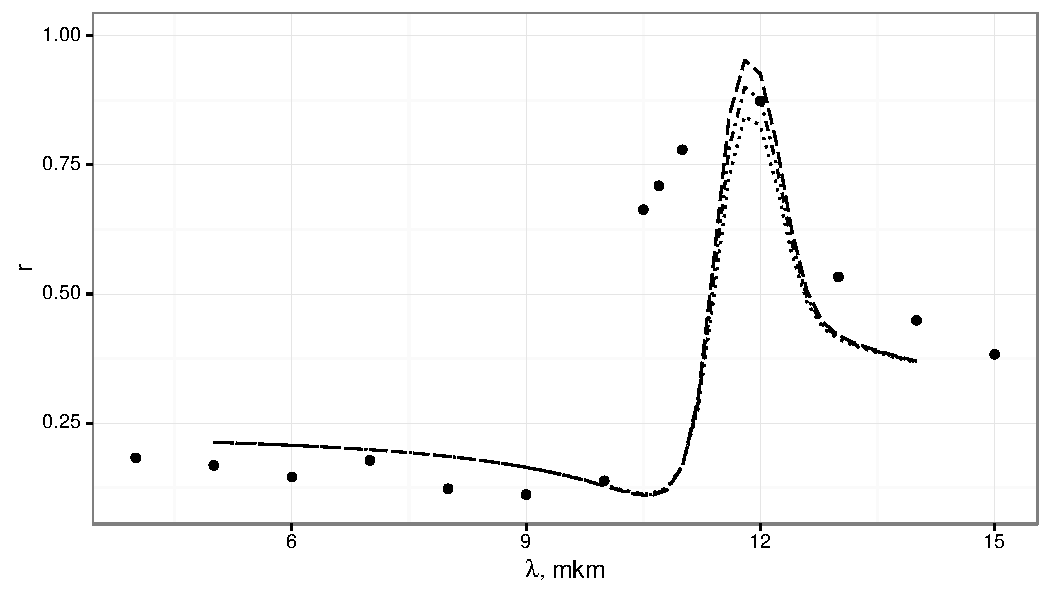
\includegraphics[width=\maxwidth]{figure/rgraph53-1} \caption[График спектров отражения]{График спектров отражения. Подбор коэффициента }\label{fig:rgraph53}
\end{figure}


\end{knitrout}

Наилучшее совпадение  при $\gamma = 3.4 \cdot 10^6$.  Тогда $\gamma/w_0 = \ensuremath{1.43\times 10^{-7}} $




%---------------------------------------------------------------
% PART5 _==================================================================
\textbf{5.} Сравнение экспериментального коэффициента отражения Ge с расчетным

Принимаем $n=4, k \ll 1 $

$$r = \frac{(n-1)^2+k^2}{(n+1)^2+k^2} = \frac{(n-1)^2}{(n+1)^2}=0.36$$

Результат усреднения экспериментальных значений: 0,46. Такое расхождение может быть объяснено путём учёта многократных отражений.


\begin{knitrout}
\definecolor{shadecolor}{rgb}{0.969, 0.969, 0.969}\color{fgcolor}\begin{figure}[!h]
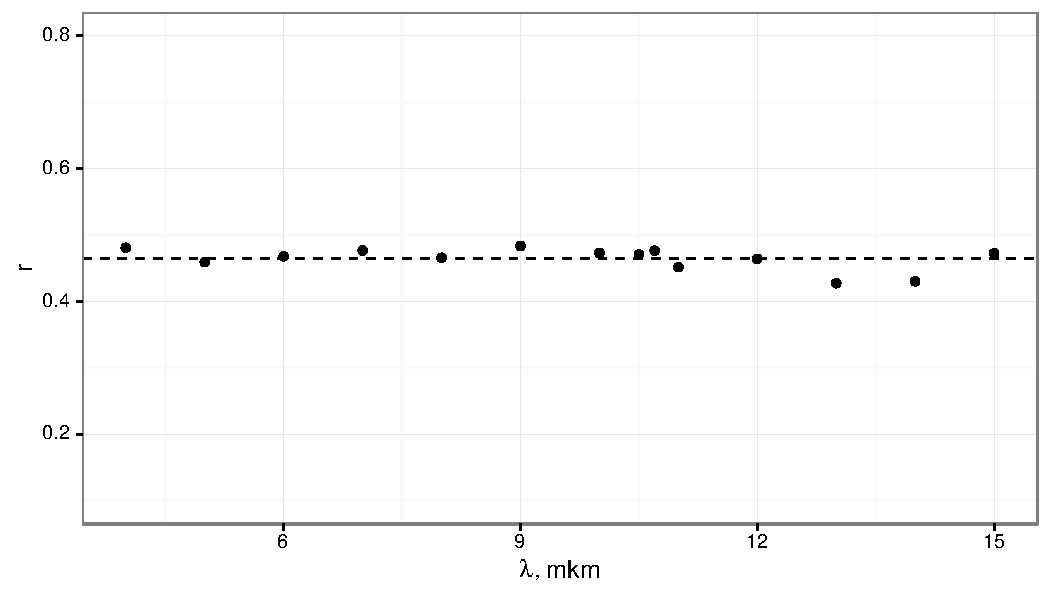
\includegraphics[width=\maxwidth]{figure/rgraph54-1} \caption[Среднее значение коэффициента отражения германия]{Среднее значение коэффициента отражения германия}\label{fig:rgraph54}
\end{figure}


\end{knitrout}

%-------------------------------------------------------------------------------
%__Conclusion__==================================================================
\clearpage
\section*{Вывод}

В результате работы были проведены исследования двух образцов: SiC и Ge
Модель классического осциллятора действительно может с высокой точностью описывать явление решеточного отражения. Данная модель после подбора коэффициентов показала  совпадение расчетных значений с экспериментальными в исследуемой области. Была получена интепретация спектра для SiC через коэффициенты: $\varepsilon_0 = 9.73$, $\varepsilon_{\infty} =   7.52$, $\omega_0 = 23.80 \cdot 10^{12} Hz$, $\gamma/w_0 = \ensuremath{1.43\times 10^{-7}} $

Теоретически рассчитанный коэффициент r(Ge) меньше среднего экспериментального на $\sim 20\%$. Однако, при расчёте коэффициента не было учтено многократное отражение света от границ образца. Расхождение может быть объяснено погрешностями при измерении и аппроксимации, несовершенством границ кристалла, а так же ненулевым показателем поглощения, которым мы пренебрегли в расчетах. 


%__Appendix__===============================================
%\appendix
\chapter*{Приложение} \label{Appendix}
\section*{Входные данные}

\begin{kframe}


{\ttfamily\noindent\bfseries\color{errorcolor}{\#\# Error in setwd("{}\textasciitilde{}/Documents/Labs/lab08"{}): cannot change working directory}}\end{kframe}% latex table generated in R 3.2.2 by xtable 1.8-0 package
% Mon Feb 29 00:33:39 2016
{\small
\begin{longtable}{|r|r|rrr|}
  \hline
 & l & Al & SiC & Ge \\ 
  \hline
1 & 4.00 & 249.70 & 46.60 & 122.50 \\ 
  2 & 5.00 & 179.50 & 30.80 & 84.10 \\ 
  3 & 6.00 & 90.70 & 13.50 & 43.30 \\ 
  4 & 7.00 & 77.10 & 14.00 & 37.50 \\ 
  5 & 8.00 & 58.50 & 7.35 & 27.80 \\ 
  6 & 9.00 & 33.60 & 3.83 & 16.57 \\ 
  7 & 10.00 & 22.30 & 3.15 & 10.76 \\ 
  8 & 10.50 & 17.45 & 11.81 & 8.38 \\ 
  9 & 10.70 & 16.60 & 12.02 & 8.07 \\ 
  10 & 11.00 & 13.37 & 10.63 & 6.16 \\ 
  11 & 12.00 & 8.30 & 7.40 & 3.93 \\ 
  12 & 13.00 & 5.00 & 2.72 & 2.18 \\ 
  13 & 14.00 & 2.62 & 1.20 & 1.15 \\ 
  14 & 15.00 & 1.10 & 0.43 & 0.53 \\ 
   \hline
\hline
\caption{Входные данные} 
\end{longtable}
}






%====================================================================
\end{document}
